\chapter{Các phương pháp phân loại}
%\addcontentsline{toc}{chapter}{Chương 2 - Trình bày luận văn}
\label{Chapter2}

\section{Phương pháp phân chia miền}
\subsection{Giới thiệu}
\hspace{10mm}Phương pháp phân chia miền được thực hiện bằng cách tái phân bổ các đối tượng. Bắt đầu từ miền khởi tạo, phương pháp này dịch chuyển đối tượng từ phân nhóm này sang phân nhóm khác. Phương pháp này thường đòi hỏi số lượng phân nhóm phải được thiết lập bởi người dùng. Do số lượng phân nhóm được thiết lập bởi ban đầu nên kết quả thường không được tối ưu. Vì vậy, phương pháp này cần một quá trình liệt kê đầy đủ tất cả các phân vùng có thể. \\
\hspace*{10mm}Nhưng việc liệt kê đầy đủ tất cả các phân vùng có thể không phải là điều khả thi. Thay vào đó, các thuật toán heuristics được sử dụng để có hiệu quả tương đương. Các thuật toán heuristics thường được áp dụng trong các hình thức tối ưu hóa vòng lặp. Nói cách khác, việc tái phân bổ các đối tượng theo vòng lặp để phân phối các các đối tượng trong $k$ phân nhóm.\\
\hspace*{10mm}Giả sử chúng ta có một cơ sở dữ liệu có $n$ đối tượng.  Mục tiêu là phân chia $n$ đối tượng vào $k$ miền cho trước. Và mỗi một miền được chia thể hiện một phân nhóm và $k \leq n$. Điều đó có nghĩa là sẽ phân loại dữ liệu vào $k$ nhóm dể thỏa mãn các điều sau:\\
\begin{enumerate}
\vspace{-10mm}
\item[•]Mỗi nhóm có ít nhất một đối tượng.
\item[•]Mỗi đối tượng phải nằm trong một nhóm duy nhất.
\end{enumerate}

\subsection{Thuật toán K-means}
%\hspace{10mm}Thuật toán K-means chỉ hoạt động dựa trên dữ liệu đầu vào là số. Mỗi phân nhóm kết hợp với một điểm trung tâm(tính bằng cách trung bình hóa). Mỗi một đối tượng được xem như là một điểm và được gắn vào phân nhóm gần điểm trung tâm nhất. Thuật toán K-means thường sử dụng công thức tính khoảng cách Euclid để đo khoảng cách giữa hai điểm. Sau đây, tôi trình bày các bước để tạo thành các phân nhóm dựa vào thuật toán K-means:\\
%\vspace{-10mm}
\begin{enumerate}
\item[•]Đầu tiên, ta chọn $k$ phân nhóm và tính $k$ điểm trung tâm ngẫu nhiên.
\item[•]Thuật toán sẽ gán mỗi đối tượng ở gần phân nhóm trung tâm nhất.
\item[•]Điểm trung tâm của phân nhóm sẽ được tính lại dựa vào các đối tượng được gắn vào.
\item[•]Thuật toán sẽ lặp cho đến khi nào mà tiến đến hội tụ(đặt ngưỡng cho mỗi phân nhóm được gán).
\end{enumerate}

\begin{figure}[htp]
\centering
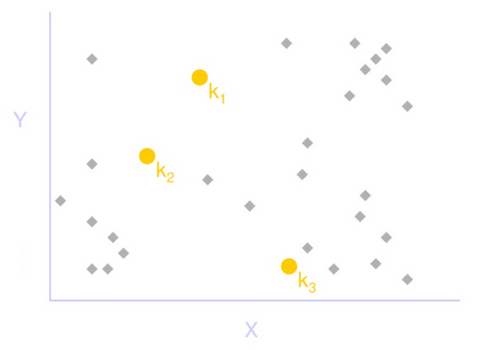
\includegraphics{Images/k_means_01}
\caption{Khởi tạo 3 điểm trung tâm ngẫu nhiên}
\label{fig:k_means_01}
\end{figure}

\begin{figure}[htp]
\centering
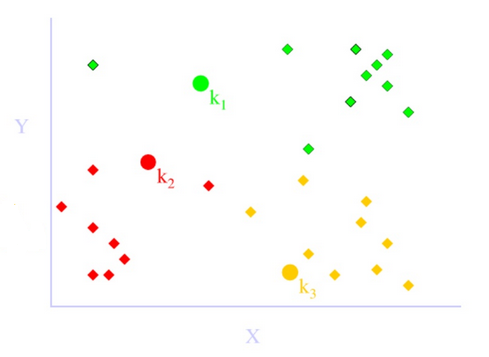
\includegraphics{Images/k_means_02}
\caption{Gán từng điểm đến điểm trung tâm gần nhất}
\label{fig:k_means_02}
\end{figure}

\begin{figure}[htp]
\centering
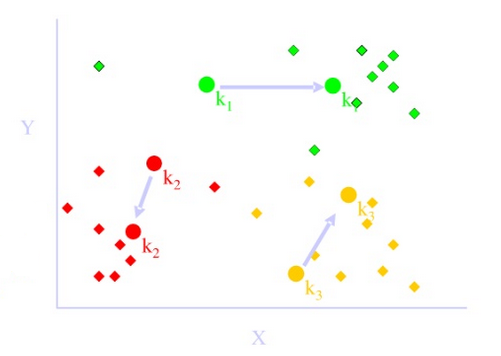
\includegraphics{Images/k_means_03}
\caption{Dịch chuyển điểm trung tâm đến điểm trung bình của phân nhóm}
\label{fig:k_means_03}
\end{figure}

\begin{figure}[htp]
\centering
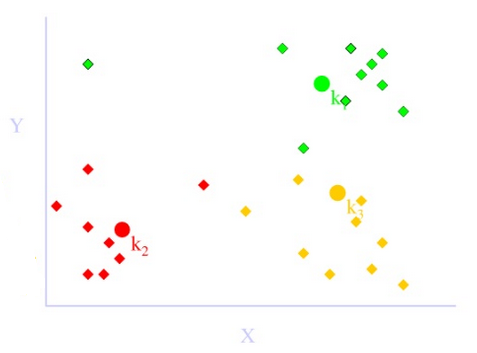
\includegraphics{Images/k_means_04}
\caption{Gán lại từng điểm đến điểm trung tâm mới}
\label{fig:k_means_01}
\end{figure}

\begin{figure}[htp]
\centering
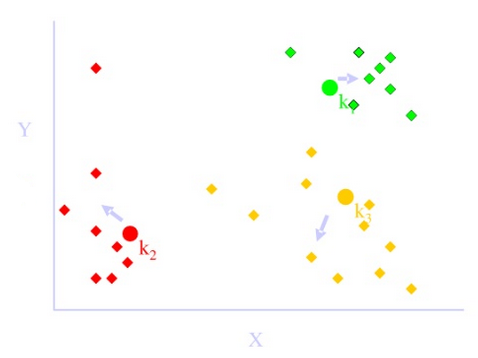
\includegraphics{Images/k_means_05}
\caption{Tính lại điểm trung tâm}
\label{fig:k_means_01}
\end{figure}

\clearpage
\section{Phương pháp dựa vào mật độ}
\subsection{Giới thiệu}
\hspace{10mm}Phương pháp này phân loại dựa vào mật độ của các điểm. Ý tưởng cơ bản là cứ tiếp tục phát triển phân nhóm cho đến mật độ của hàng xóm vượt ngưỡng. Nghĩa là mỗi điểm thuộc về một phân nhóm, bán kính của phân nhóm phải chứa ít nhất một số điểm. Các phân nhóm có mật độ dày đặc được chia cắt bởi các phân nhóm có mật độ thấp. Mật độ các điểm của phân nhóm tạo thành nên các hình thù ngẫu nghiên của phân nhóm đó.\\

\subsection{Các thuật toán}
\subsubsection{Thuật toán DBSCAN}
\begin{enumerate}
\item[•]Mật độ là số điểm nằm trong vùng bán kính $\varepsilon$ nhất định(viết tắt là $Eps$).
\item[•]Hàng xóm nằm trong phạm vi bán kính $\varepsilon$ của một đối tượng được gọi là $\varepsilon$-neighborhood của đối tượng đó: $ N_{\varepsilon}(p) : \{q\, |\, d(p,q)\, \leq\, \varepsilon\} $.
\item[•]$MinPts$ là số điểm tối thiểu dùng thể hình thành vùng mật độ.
\item[•]Một đối tượng $p$ được xem là mật độ khả chuyển trực tiếp từ đối tượng $q$ nếu $p$ nằm trong phạm vi $\varepsilon$-neighborhood của $q$ và $q$ được xem là đối tượng hạt nhân.
\item[•]Một đối tượng $p$ được xem là mật độ khả chuyển từ đối tượng $q$ nếu có một chuỗi các đối tượng $p_1, \ldots, p_n$ với $p_1=p$ và $p_n=q$ thỏa mãn $p_{i + 1}$ là mật độ khả chuyển trực tiếp từ $p_i$.
\item[•]Một đối tượng được xem là mật độ kết nối đến $p$ đối với $\varepsilon$ và $MinPts$ nếu ở đó có một đối tượng $o$ mà cả $p$ và $q$ đều mật độ khả chuyển từ $o$.
\item[•]Điểm biên giới là điểm có ít hơn $MinPts$ trong phạm vi $Eps$, nhưng là trong hàng xóm của điểm hạt nhân.
\item[•]Phân nhóm dựa vào mật độ là một tập hợp của những đối tượng kết nối mật độ cực đại đối với mật độ khả chuyển.
\item[•]Điểm nhiễu là điểm cô lập.
\end{enumerate}

\begin{figure}[htp]
\centering
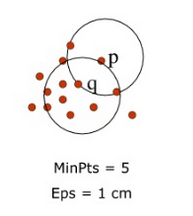
\includegraphics{Images/Density_01}
\caption{Mật độ khả chuyển trực tiếp}
\label{fig:Density_01}
\end{figure}

\begin{figure}[htp]
\centering
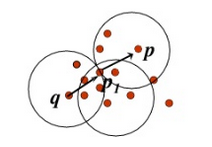
\includegraphics{Images/Density_02}
\caption{Mật độ khả chuyển}
\label{fig:Density_02}
\end{figure}

\begin{figure}[htp]
\centering
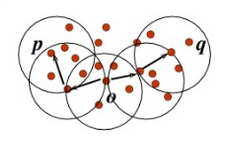
\includegraphics{Images/Density_03}
\caption{Mật độ kết nối}
\label{fig:Density_03}
\end{figure}

\begin{figure}[htp]
\centering
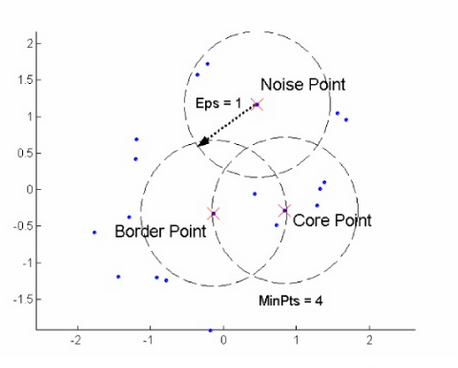
\includegraphics{Images/Density_04}
\caption{Điểm hạt nhân, điểm biên giới, điểm nhiễu}
\label{fig:Density_04}
\end{figure}

\clearpage
\underline{Thuật toán:}
\begin{enumerate}
\item[]Chọn ngẫu nhiên điểm $p$.
\item[]Truy vấn tất cả những điểm mật độ khả chuyển từ $p$ với $Eps$ và $MinPts$ cho trước.
\item[]Nếu $p$ là điểm hạt nhân, một phân nhóm mới được hình thành.
\item[]Nếu $p$ là điểm biên giới, không có điểm nào là mật độ khả chuyển từ $p$ và DBSCAN thăm điểm tiếp theo của cơ sở dữ liệu.
\item[]Tiếp tục tiến trình cho đến khi tất cả những điểm đều được duyệt.
\end{enumerate}

\subsubsection{Thuật toán OPTICS}
\hspace{10mm}Đây là thuật toán mở rộng từ DBSCAN, sắp xếp điểm để xác định cấu trúc của phân nhóm. Thuật toán tạo ra thứ tự đặc biệt của dữ liệu đối với cấu trúc phân nhóm dựa vào mật độ. Thứ tự phân nhóm chứa thông tin tương ứng với những phân nhóm dựa vào mật độ tương tự miền rộng của thiết lập tham số. Đây là thuật toán hay cho cả việc tự động và tính tương tác trong việc phân tích phân nhóm. Thuật toán này có thể được thể hiện bằng kỹ thuật đồ họa hoặc hình ảnh.\\
\begin{enumerate}
\vspace{-10mm}
\item[]$k$ : số miền
\item[]$N$ : số điểm
\item[]$O(N*logN)$ : độ phức tạp của thuật toán
\item[]Khoảng cách hạt nhân của một đối tượng $p$ là giá trị $\varepsilon$ nhỏ nhất thỏa mãn $\varepsilon$-neighborhood của $p$ có ít nhất một đối tượng $MinPts$.
\begin{align*}
Core-distane_{\varepsilon, MinPts}(p) =& undefined\; if\; card(N_\varepsilon(p))\,\leq\, MinPts \\
=& MinPts-distance(p), otherwise
\end{align*}
\item[]Khoảng cách khả chuyển của đối tượng $p$ từ đối tượng hạt nhân là giá trị bán kính nhỏ nhất mà $p$ mật độ khả chuyển từ $q$.
\begin{align*}
Reachability-distance_{\varepsilon, MinPts}(p,q) =& undefined\; if\; q is not a core object \\
=& max(core-distance(q), distance(q,p)), otherwise
\end{align*}
\end{enumerate}

\begin{figure}[htp]
\centering
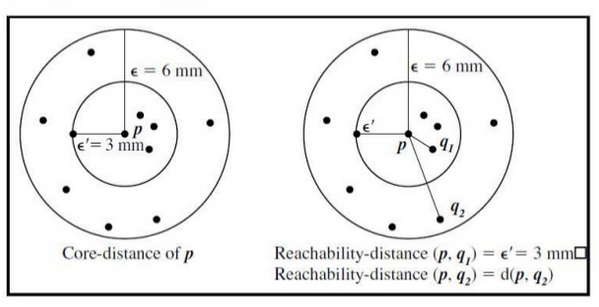
\includegraphics{Images/Optics_01}
\caption{Các thuật ngữ trong OPTICS}
\label{fig:Optics_01}
\end{figure}


\subsubsection{Thuật toán DENCLUE}
\hspace{10mm}Đây là thuật toán được giới thiệu bởi Hinnerburg và Keim, sử dụng hàm mật độ thống kê.\\
\begin{align*}
f_{Gaussian}(x,y) \, =& \, e^{\frac{d(x,y)^2}{2{\sigma}^2}} \; influence\, of\, y\, on\, x\\
f^D_{Gaussian}(x) \, =& \, \sum_{i=1}^N \, e^{-\frac{d(x,y)^2}{2{\sigma}^2}} \; total\, influence\, on\, x \\
\bigtriangledown \, f^D_Gaussian(x, x_i) \, =& \, \sum_{i=1}^N \, (x_i - x) \cdot e^{-\frac{d(x,y)^2}{2{\sigma}^2}} \; gradient\, of\, x\, in\, the\, direction\, of\, x_i
\end{align*}
\hspace{10mm}Thuật toán có nền tảng hoàn toàn là các công thức toán học. Thuật toán thích hợp cho các tập dữ liệu có độ nhiễu lớn. Nó còn cho phép mô tả toán học chặt chẽ của hình dạng phân nhóm ngẫu nhiên trong tập dữ liệu có số chiều cao. Điều quan trọng là thuật toán này nhanh hơn so với các thuật toán đang tồn tại(như DBSCAN). Tuy nhiên, đây là thuật toán đòi hỏi cần có nhiều tham số thiết lập.\\
\hspace*{10mm}Sau đây, ta cùng nhau đánh giá bản chất kỹ thuật của thuật toán DENCLUE. Thuật toán sử dụng mạng lưới ô nhưng chỉ giữ thông tin cho ô chứa dữ liệu điểm. Các ô này được quản lý và truy xuất dưới dạng cấu trúc cây. Các hàm tác động mô tả độ tác động của điểm dữ liệu trong phạm vi hàng xóm. Và mật độ của khoảng trống dữ liệu nếu bị vượt quá có thể tính như là tổng của hàm tác động của tất cả điểm dữ liệu.\\
\hspace*{10mm}Phân nhóm có thể xác định một cách toán học bằng việc xác định điểm hấp dẫn mật độ. Điểm hấp dẫn mật độ là cục bộ lớn nhất của toàn hàm mật độ. Trung tâm phân nhóm được xác đinh bằng cách gán những điểm mật độ đến điểm hấp dẫn mật độ. Những điểm hấp dẫn mật độ kết nối tạo thành đường vượt qua ngưỡng tạo nên hình thù ngẫu nhiên của phân nhóm.\\

%\subsubsection{Thuật toán CLIQUE}

\section{Phương pháp dựa vào lưới tọa độ}
\subsection{Giới thiệu}
\hspace{10mm}Đây là thuật toán sử dụng mạng lưới cấu trúc dữ liệu đa phân giải. Thông thường, bài toán phân loại trên dữ liệu lớn có độ tính toán phức tạp cao. Tuy nhiên, thuật toán này có ưu điểm lớn là giảm được độ phức tạp khi tính toán, đặc biệt là dữ liệu lớn. Hướng tiếp cận của thuật toán này cũng cũng khác so với các thuật toán phân loại thường gặp. Thuật toán này không tập trung vào điểm dữ liệu mà vào giá trị xung quanh điểm dữ liệu. 

Các thuật toán dựa vào lưới tọa độ bao gồm các bước:
\begin{enumerate}
\item[•]Tạo cấu trúc mạng lưới, phân chia không gian dữ liệu vào số ô hữu hạn.
\item[•]Tính toán mật độ cho mỗi ô.
\item[•]Sắp xếp thứ tự các ô dựa vào mật độ mỗi ô.
\item[•]Xác định phân nhóm trung tâm.
\item[•]Duyệt các ô hàng xóm.
\end{enumerate}

\subsection{Các thuật toán}
\subsubsection{Thuật toán STING}
\hspace{10mm}Đây là thuật toán tiếp cận theo hướng mạng lưới thông tin thống kê. Vùng thông tin không gian được chia thành các ô hình chữ nhật. Các ô này có nhiều cấp độ tương ứng với cấp độ phan giải khác nhau. Mối ô tại cấp độ cao được phân chia thành những ô nhỏ hơn ở cấp độ thấp hơn kế cận. Thông tin thống kê của mỗi ô được tính toán và lưu trữ trong trước và thường dùng để truy vấn.

\clearpage
\begin{figure}[htp]
\centering
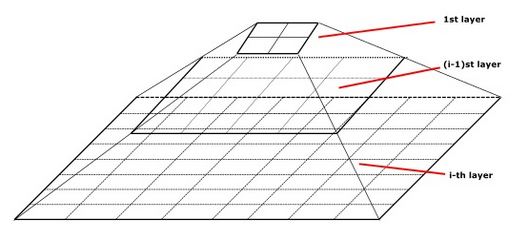
\includegraphics{Images/Sting_01}
\caption{Hình ảnh sơ bộ về thuật toán STING}
\label{fig:Sting_01}
\end{figure}

\hspace{10mm}Tham số sử dụng trong các ô tầng cao có thể tính được từ các tham số của ô tầng thấp. Các tham số đó bao gồm : count, mean, s, min, max và các dạng phân phối. Thuật toán tiếp cận theo hướng từ trên xuống để có thể trả lời câu hỏi truy vấn. Thuật toán bắt đầu từ lớp được chọn trước, thường là một số lương nhỏ các ô. Mỗi ô trong cấp độ hiện tại được tính toán độ tin cậy.\\

\underline{Thuật toán STING}
\begin{enumerate}
\item[•]Thuật toán xóa bỏ những ô không liên quan sau khi suy xét.
\item[•]Khi thuật toán kết thúc lớp hiện tại, tiếp tục đến lớp kế tiếp thấp hơn.
\item[•]Quá trình này lặp lại cho đến khi nào chạy đến lớp cuối cùng. 
\end{enumerate}

\underline{Ưu điểm}
\begin{enumerate}
\item[•]Truy vấn phụ thuộc, dễ dàng tính toán song song, cập nhật tăng trưởng.
\item[•]$O(K)$ với $K$ là số lượng ô của mạng lưới ở cấp độ thấp nhất.
\end{enumerate}

\underline{Khuyết điểm }: 
tất cả các biên giới phân nhóm có thể là chiều ngang hoặc dọc, và không thể tìm thấy đường chéo.

\subsubsection{Thuật toán CLIQUE}
\hspace{10mm}CLIQUE có thể được xem như phương pháp dựa vào mật độ lẫn mạng lưới. Nó có thể chia mỗi miền vào số lượng giống nhau về độ đo chiều dài bằng nhau. Đồng thời, nó cũng chia không gian dữ liệu thành $m$ miền vào những đơn vị hình chữ nhật mà không bị đè lên. Một đơn vị được xem là dày đặc nếu tỉ lệ giữa số điểm tổng cộng chứa một đơn vị vượt quá tham số mẫu đầu vào. Một phân nhóm là tập cực đại của đơn vị mật độ kết nối trong không gian con.\\

Những điểm chính trong thuật toán CLIQUE:
\begin{enumerate}
\item[•]Phân loại không gian dữ liệu và tìm số điểm mà nằm trong mỗi ô của phân miền.
\item[•]Xác định các không gian con mà chứa các phân nhóm sử dụng độ ưu tiên Apriori.
\item[•]Xác định phân nhóm:
\begin{enumerate}
\item[-]Xác định mật độ của đơn vị trong tất cả không gian con.
\item[-]Xác định mật độ kết nối của đơn vị trong tất cả không gian con.
\end{enumerate}
\item[•]Tạo ra mô tả tối thiểu cho các phân nhóm:
\begin{enumerate}
\item[-]Xác định vùng cực đại mà chứa phân nhóm của mật độ kết nối của đơn vị cho mỗi phân nhóm.
\item[-]Xác định độ phủ tối tiểu cho mỗi phân nhóm.
\end{enumerate}
\end{enumerate}

\begin{figure}[htp]
\centering
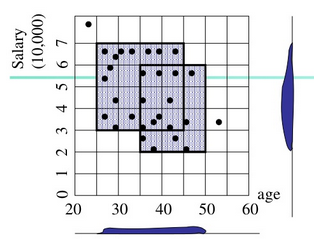
\includegraphics{Images/Clique_01}
\caption{Đồ thị về lương và tuổi}
\label{fig:Clique_01}
\end{figure}

\begin{figure}[htp]
\centering
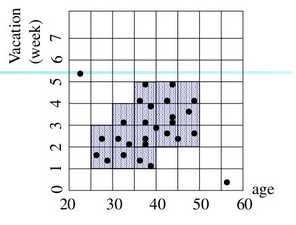
\includegraphics{Images/Clique_02}
\caption{Đồ thị về kì nghỉ và tuổi}
\label{fig:Clique_02}
\end{figure}

\begin{figure}[htp]
\centering
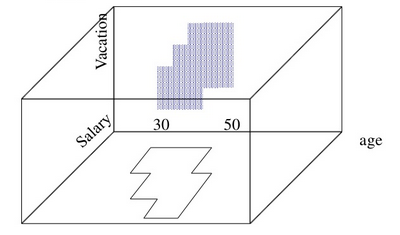
\includegraphics{Images/Clique_03}
\caption{Đồ thị kết quả}
\label{fig:Clique_03}
\end{figure}

\underline{Điểm mạnh }:
\begin{enumerate}
\item[•]Tự động tìm các không gian con của số chiều cao nhất thỏa mãn các phân nhóm mật độ cao tồn tại trong các không gian này.
\item[•]Mạnh mẽ trong việc sắp đặt dữ liệu đầu vào và không có ước đoán dữ liệu phân phối chính tắc.
\item[•]Co giãn tuyến tính với độ lớn của đầu vào và có độ co giãn tốt như số lượng miền trong dữ liệu gia tăng.
\end{enumerate}

\underline{Điểm yếu }: Độ chính các của kết quả phân loại có thể giảm do chí phí của phương pháp.
%\subsubsection{Thuật toán WaveCluster}
\section{Phương pháp dựa vào mô hình}
\subsection{Giới thiệu}
\hspace{10mm} Đây là phương pháp dựa vào giả thiết dữ liệu được tạo ra bởi sự pha trộn của các phân phối xác suất. Trong phương pháp này, một mô hình được giả thiết cho mỗi phân nhóm đề tìm sự thích hợp tốt nhất của dữ liệu cho mô hình đã cho. Hay nói cách khác, thuật toán cố gắng tối ưu độ tương thích giữa dữ liệu và mô hình toán học. Phương pháp này định vị phân nhóm bằng hàm mật độ phân loại. Đồng thời, nó phản ánh phân phối của không gian của những điểm dữ liệu.

\subsection{Thuật toán phân loại cực đại mong đợi}
\hspace{10mm}Đây là thuật toán phổ biến để tinh chế lại vòng lặp, là phần mở rộng của $K-means$. Gán mỗi đối tượng vào một phân nhóm tương ứng với độ lớn phân phối xác suất. Độ trung bình mới được tính dựa vào cách đo độ lớn. Thuật toán hội tụ nhanh nhưng không được tối ưu toàn cục.\\
\hspace*{10mm}Ý tưởng cơ bản là thuật toán bắt đầu với ước lượng khởi tạo có tham số vector. Sau đó, nó lặp lại cách ghi mẫu đối với sự pha trộn mật độ tạo ra bởi tham số vector. Mẫu được ghi lại thường sử dụng để cập nhật tham số. Những mẫu thuộc về phân nhóm giống nhau nếu chúng đặt bởi lượt ghi trong thành phần riêng biệt.\\
\underline{Thuật toán }:
\begin{enumerate}
\item[•]Khởi tạo ngẫu nhiên $k$ điểm trung tâm.
\item[•]Tinh chế lại các phân nhóm dựa vào 2 bước:
\begin{enumerate}
\item[-]Bước mong đợi : gắn mỗi điểm dữ liệu $X_i$ cho phân nhóm $C_i$ với xác suất sau
\begin{equation*}
P(X_i \, \in C_k) \, = \, p(C_k|X_i) = \frac{p(C_k)p(X_i|C_k)}{p(X_i)} 
\end{equation*}
với $p(X_i|C_k)\,=\,N(m_k,E_k(x_i))$ theo phân phối chuẩn. Bước này tính ra xác suất của phân nhóm thành viên $x_i$ cho mỗi $C_k$.
\item[-]Bước cực đại : ước lượng mô hình tham số
\begin{equation*}
m_k\,=\,\frac{1}{N}\sum^N_{i=1} \frac{X_i P(X_i \in C_k)}{\sum_j P(X_i \in C_j)}
\end{equation*}
\end{enumerate}
\end{enumerate}

%\section{Phương pháp dựa vào ràng buộc}

%\section{Giới thiệu về Goodman-Kruskal}
%
%aaaaaaaaaaa
%%Các tiểu mục của luận văn được trình bày và đánh số thành nhóm chữ số, nhiều nhất gồm bốn chữ số với số thứ nhất chỉ số chương (ví dụ: 4.1.2.1. chỉ tiểu mục 1 nhóm tiểu mục 2 mục 1 chương 4).
%%Tại mỗi nhóm tiểu mục phải có ít nhất hai tiểu mục, nghĩa là không thể có tiểu mục 2.1.1 mà không có tiểu mục 2.1.2 tiếp theo.
%
%\section{Thuật toán Hierarchial Co-clustering}
%\subsection{Sử dụng Goodman-Krusal với Hierarchial Co-Clustering}
%ggggggggggg
%%Việc đánh số bảng biểu, hình vẽ, phương trình phải gắn với số chương; ví dụ hình 3.4 có nghĩa l hình thứ 4 trong Chương 3.
%%Mọi đồ thị, bảng biểu lấy từ các nguồn khác phải được trích dẫn đầy đủ. Nguồn được trích dẫn phải được liệt kê chính xác trong danh mục Tài liệu tham khảo.
%%Đầu đề của bảng biểu ghi phía trên bảng, đầu đề của hình vẽ ghi phía dưới hình.
%%Thông thường, những bảng ngắn và đồ thị phải đi liền với phần nội dung đề cập tới các bảng và đồ thị này ở lần thứ nhất.
%%Các bảng dài có thể để ở những trang riêng nhưng cũng phải tiếp theo ngay phần nội dung đề cập tới bảng này ở lần đầu tiên.
%\subsection{Các thuật toán}
%jjjjjjjjjjjjj
%%Các bảng rộng vẫn nên trình bày theo chiều đứng dài 297mm của trang giấy, chiều rộng của trang giấy có thể hơn 210mm.
%%Chú ý gấp trang giấy sao cho số và đầu đề của hình vẽ hoặc bảng vẫn có thể nhìn thấy ngay mà không cần mở rộng tờ giấy.
%%Tuy nhiên hạn chế sử dụng các bảng quá rộng này.
%%
%%Đối với những trang giấy có chiều đứng hơn 297mm (bản đồ, bản vẽ,...) thì có thể để trong một phong bì cứng đính bên trong bìa sau của luận văn.
%%Các hình vẽ phải sạch sẽ bằng mực đen để có thể sao chụp lại; có đánh số và ghi đầy đủ đầu đề, cỡ chữ phải bằng cỡ chữ sử dụng trong văn bản luận văn.
%%Khi đề cập đến các bảng biểu và hình vẽ phải nêu rõ số của hình và bảng biểu đó, ví dụ ``... được nêu trong Bảng 4.1'' hoặc ``xem Hình 3.2'' mà không được viết ``… được nêu trong bảng dưới đây'' hoặc ``trong đồ thị của X và Y sau''.
%%
%%Việc trình bày phương trình toán học trên một dòng đơn hoặc dòng kép tùy ý, tuy nhiên phải thống nhất trong toàn luận văn.
%%Khi ký hiệu xuất hiện lần đầu tiên thì phải giải thích và đơn vị tính phải đi kèm ngay trong phương trình có ký hiệu đó.
%%Nếu cần thiết, danh mục của tất cả các ký hiệu, chữ viết tắt và nghĩa của chúng cần được liệt kê và để ở phần đầu của luận văn.
%%Tất cả các phương trình cần được đánh số và để trong ngoặc đơn đặt bên phía lề phải.
%%Nếu một nhóm phương trình mang cùng một số thì những số này cũng được để trong ngoặc, hoặc mỗi phương trình trong nhóm phương trình (5.1) có thể được đánh số là (5.1.1), (5.1.2), (5.1.3).
%
